\documentclass[10pt]{article}
\usepackage[utf8]{inputenc}
\usepackage[T1]{fontenc}
\usepackage[margin=1in]{geometry}
\usepackage{booktabs}
\usepackage{amsmath,amssymb}
\usepackage{graphicx}
\usepackage{caption}
\usepackage{microtype}
\usepackage[hidelinks]{hyperref}
\usepackage{natbib}
\bibliographystyle{plainnat}

\captionsetup{font=small,labelfont=bf}
\setlength{\parskip}{2pt}

\title{Adding a reusable representation beside a fixed prediction service:\\
what coalition-conditioned erasure buys, and what it does not}
\author{}
\date{Revision of 2026-09-17. Branch \texttt{research/pcrl-evidence-paper-v1}.}

\begin{document}
\maketitle

\begin{abstract}
An organisation already publishes a prediction service: fixed probability vectors that downstream
recipients consume and cannot be asked to re-accept. We ask whether it can add a \emph{second},
reusable representation for one recipient without changing a single published number, while limiting
what that recipient---and a coalition of recipients---can newly infer about sex and race. The
mechanism we study keeps the teacher information the published outputs do not explain and chooses
directions by maximising linear reconstruction of that residual minus conditional-moment penalties,
conditioning on the released service probabilities through cross-fitted nuisance models. Penalties
can be local to one recipient or specific to a coalition's joint view. We evaluate eight penalty
settings against five frozen adversarially trained channels and a no-channel baseline on California
ACS, then transport the entire frozen 14-interface slate to a locked, previously unused survey year.
Four findings. (i) Exact service preservation is structural and holds bitwise on all 210 released
views; it does not imply stable service accuracy, which moves by $\pm0.014$ nats across one year.
(ii) On the sealed evaluation the coalition-conditioned penalty does what it claims: it lowers
additional sensitive recovery against both an equal-strength and an equal-total-mass local control,
under simultaneous 95\% intervals and both weightings, satisfying a rule the development year had
failed. (iii) That rule is a one-sided constraint on a \emph{point} estimate, and we show the
interval evidence does \emph{not} establish non-inferiority at the same $0.001$ margin---zero of four
comparisons, under any procedure we computed. (iv) The mechanism nevertheless loses: under identical
attacks it is significantly worse than a frozen adversarially trained channel of the same width on
all four sensitive endpoints under both weightings, and we show this ordering survives matching the
two channels on average utility, in both directions. We report an evaluation contribution and a
negative method result, and we are explicit about which of our own earlier claims this revision
withdraws.
\end{abstract}

\section{What this paper is}
\label{sec:contribution}

A service that already publishes predictions can hand one recipient extra features built only from
what those predictions leave unexplained, and can steer those features away from directions that
would let that recipient---or that recipient plus a colluding one---guess sex or race better than
the published predictions already allow. We show the steering knob works on a sealed new year of
data, that it is not competitive with an adversarially trained channel of the same size, and that
the negative verdict is robust to matching the two on average utility. The useful output is
therefore the problem formulation and the evaluation design, plus a negative method result. It is
not a deployable mechanism, and we do not present it as one.

We also correct our own record. Section~\ref{sec:withdrawn} lists every claim this revision
withdraws or narrows, with the evidence. No number changed: all 90 pre-declared endpoints reproduce
under an independently written scorer to $1.1\times10^{-15}$.

\section{Threat model and interface}
\label{sec:interface}

Each person has covariates $X$, sensitive attributes $S$ (sex, 2 classes; race, 9 classes) and task
labels. Two frozen services exist: $H_A(X)\in[0,1]^4$, the income-over-\$50k and employment
probability vectors released to recipient A, and $H_B(X)\in[0,1]^2$, public coverage, released to
recipient B. A mechanism may add a channel $Z\in\mathbb{R}^{16}$ \emph{for A only}. Views: A sees
$(H_A,Z)$; B sees $H_B$; the coalition AB sees $(H_A,Z,H_B)$.

The policy authorises A for income, employment and residence, B for coverage and commute, and
forbids sex and race everywhere, coverage and commute for A, and income, employment and residence
for B---eleven forbidden roles. The adversary holds labelled data from the release year, fits fixed
attack families on its own pool, selects on a validation pool, and sees only its legal view. Every
published function, including the preprocessing, the released map and the neural arms' public
auxiliary heads, is in scope, and coalition attacks may use any legal projection of A's and B's
candidates.

\textbf{The A-only limitation is real and bounds every claim below.} Only one recipient receives a
channel. Nothing here demonstrates joint optimisation of channels for several recipients, and the
coalition penalty is a constraint on one channel given another recipient's fixed view, not a
multi-channel design.

\section{Why the published outputs are retained}
\label{sec:retained}

The constraint that makes this problem different from representation learning is that
$H_A$ and $H_B$ have already been published. Downstream consumers have built on those exact numbers;
a revision is a migration, not a deployment. So the mechanism may append but not modify:
$Z$ is concatenated to $H_A$ and never mixed into it. Exact preservation is then \emph{structural}
rather than measured---there is no perturbation whose size must be bounded---and we verify it
bitwise on every released view rather than certifying it statistically.

Two things this does not give us. It does not mean the service stays \emph{accurate}: on identical
released vectors, employment log loss rises by $0.0138$ nats and income falls by $0.0145$ between the
two years (Table~\ref{tab:criteria} discusses the probe side). And it does not constrain what the
appended channel discloses, which is the entire subject of this paper.

\section{The mechanism}
\label{sec:method}

Let $T$ be a frozen PCA32 teacher. Build $\phi(T)=[\,\text{standardised }T,\ 96 \text{ random Fourier
features}\,]$ with a median-heuristic bandwidth \citep{rahimi2007random}. Let $q_A$ be the intercept
and all degree-2 monomials in A's two positive-class service probabilities; $q_{AB}$ adds B's.
Residualise by SVD least squares, $V_0=\phi-q_A B_\phi$ and $R=T-q_A B_T$, then eigen-whiten $V_0$ to
$V$ with $V^\top V/n=I$. Utility is $U=C_{VR}C_{RV}$: for $W^\top W=I$, $\operatorname{tr}(W^\top UW)$
is exactly the training reduction in least-squares reconstruction error of the residualised teacher.
Protection matrices use household-grouped 3-fold cross-fitted multinomial-logistic nuisances $m_j$
(cross-fitting in the sense of \citealp{chernozhukov2016dml}; we claim none of that work's
orthogonality or rate guarantees for our moments)
and, for each retained basis column $b_k$,
\[
G_{jk}=\frac{1}{n_j}\sum_i V_i\, b_k(H_i)\,\bigl(\mathrm{onehot}(S_j)_i-m_j(H_i)\bigr)^{\!\top},
\qquad P_j=\textstyle\sum_k G_{jk}G_{jk}^{\top}\ \text{(trace-normalised)},
\]
averaged over local roles (basis $q_A$: sex, race, coverage), coalition roles (basis $q_{AB}$: sex,
race) and a marginal variant (constant basis). The released map is the top-16 eigenvectors of
$U_{\mathrm{norm}}-\lambda P$, giving arms S0 ($\lambda=0$), M025/M1 (marginal), L025/L1/L2 (local)
and C025/C1 (local $+$ coalition). Inference needs only $T$ and $H_A$; $H_B$ enters fitting and
auditing only.

\subsection{What is a theorem, and what is not}
\label{sec:scope}

The eigenvector step is Ky Fan's maximum principle for a \emph{fixed} empirical matrix
\citep{fan1949weyl}. It certifies nothing about the choice of features, basis, nuisances, rank or
attacker, and with $r$ fixed at 16 it can retain directions whose penalty exceeds their utility.
Selecting rank by eigenvalue sign instead is not our idea and is not new: it is SARL's Theorem 3,
OptNet-ARL's Theorem 4.1 and K-TOpt's Corollary 4.1
\citep{sadeghi2019sarl,sadeghi2021optnetarl,sadeghi2022ktopt}. We fixed $r=16$ to match the width of
the neural baselines, which is a comparison choice, not an optimum.

The moment condition is a finite subset of the $L^2$ characterisation of conditional independence
that kernel CI tests use \citep{zhang2011kci,strobl2019rcit}. Precisely, it is Lemma 2(v) of
\citet{zhang2011kci}, attributed there to Daudin: our centring on the $S$ side is algebraically
equivalent to residualising the $(Z,H)$ side, since with $\tilde f=f-\mathbb{E}[f\mid H]$ we have
$\mathbb{E}[f(Z,H)(\mathbf 1\{S=c\}-m_c(H))]=\mathbb{E}[\tilde f\cdot\mathbf 1\{S=c\}]$. The
characterisation quantifies over \emph{every} square-integrable $f$; we test
$f\in\{Z_\ell b_k(H)\}$---linear in $Z$, degree-2 in $H$, with estimated nuisances and finite
samples. Consequently vanishing fitted moments do not establish conditional independence, and a
non-zero moment may reflect nuisance error rather than leakage. Two fixtures make this concrete and
are carried in the code. An XOR channel has exactly zero marginal moment while $S=ZH$ recovers it
perfectly; it is detected by an interaction term \emph{in $H$}, so enriching the conditioning side
suffices. A magnitude channel---$(Z,S)$ uniform on $\{(-1,0),(1,0),(-2,1),(2,1)\}$ with $H$
constant---has exactly zero first moment, yet $\mathbf 1\{|Z|>1.5\}$ recovers $S$ exactly; because
$H$ is constant, \emph{no} enrichment of the conditioning side can ever see it, and only a nonlinear
function of $Z$ can ($\mathbb{E}[Z^2(S-\tfrac12)]=0.75$). The attacks that defeat our arms on ACS are
MLPs and boosted trees, i.e.\ the second kind.

With population-optimal log-loss predictors, the $H$ versus $(H,Z)$ risk difference equals
$I(S;Z\mid H)$. Our validation-selected finite attacks do not attain those infima, so the reported
differences bound it in neither direction---indeed some are negative---and mutual-information
estimation has its own formal limits \citep{mcallester2020formal}. We report no certified
information quantity. For the withholding control, an independent visible branch
$B\sim\mathrm{Bernoulli}(p)$ gives $I(S;B,Z_B\mid H)=p\,I(S;Z\mid H)$ and expected routed loss
$(1-p)L_H+p\,L_{HZ}$; the branch must be persistent, since independent re-draws would eventually
reveal $Z$.

\section{Relation to prior work}
\label{sec:related}

The closed-form line of Sadeghi, Dehdashtian and Boddeti already solves this shape of problem. SARL
\citep{sadeghi2019sarl} takes eigenvectors of a utility-minus-$\lambda$-dependence matrix; OptNet-ARL
\citep{sadeghi2021optnetarl} keeps closed-form ridge players inside a learned encoder and already
handles several sensitive attributes through several $\lambda$; K-TOpt \citep{sadeghi2022ktopt} adds
random Fourier features and evaluates on Folktables \citep{ding2021retiring}; U-FaTE
\citep{dehdashtian2024ufate} adds a \emph{conditional} penalty. Our marginal arms are, up to
parametrisation, SARL's construction on whitened random-feature residuals.

Three things differ, and we state their weight honestly. \emph{What we condition on:} U-FaTE's
conditional measure is stratification over a discrete label $Y$, and its own text scopes the
equivalence to ``when $Y$ is not a continuous label''; $H_A$ is a pair of continuous probability
vectors, so stratification is unavailable and we substitute cross-fitted nuisance residuals. $H$ is
also a \emph{released artifact} rather than the label to be predicted---a different object even
setting continuity aside. \emph{What utility means:} reconstruction of a residualised teacher rather
than dependence with a label. \emph{Recipient structure:} separate local and coalition penalties,
with only one recipient receiving a channel.

The first two are adaptations of known components, not new optimisation principles. The third we did
not find in the surveyed literature, and the nearest candidate is weaker prior art than its title
suggests: the multi-consumer information-theoretic line \citep{sankar2013utility} designs \emph{one}
sanitised release consumed by many users who differ only in private side information, with no
per-recipient release, no collusion term, and no constraint to preserve an already-published output.
Linear concept erasure \citep{belrose2023leace,holstege2025splince} addresses a different guarantee
(exact \emph{linear} erasure) on a representation the releaser owns and may edit; LEACE scopes its
guarantee to linear adversaries explicitly. Adversarial removal is known to leave recoverable
information \citep{elazar2018adversarial}, and least-privilege learning has fundamental limits
\citep{stadler2024leastprivilege}.

Two further neighbourhoods are worth separating from ours. Conditional fair representation learning
conditions on a \emph{label} for separation-style criteria
\citep{zhao2019conditional,hwa2024enforcing}, not on a released prediction, and again designs the
representation from scratch. Information-theoretic privacy gives the quantities our log-loss
endpoints relate to---leakage and utility both become mutual information under log loss
\citep{makhdoumi2014funnel}, with perfect-privacy conditions \citep{rassouli2021perfect} and
robustness of leakage measures to side information \citep{liao2019sideinfo}---but assumes a known
joint distribution and a randomised mapping, whereas our released map is deterministic and our
attacks are fitted. Task-agnostic private representation learning \citep{arevalo2024tappfl} targets
attribute inference without a known downstream task, again with no fixed prior output and one
recipient. A bounded search cannot establish novelty and we make no priority claim.

\section{Experimental design}
\label{sec:design}

California ACS one-year PUMS, ages 19--34. \emph{Development:} 2018, three household splits (seeds),
with disjoint pools for representation fitting, source validation, task fitting and validation,
attacker fitting and validation, and development evaluation. Fourteen interfaces per seed---H (no
channel), E, A0, L025, L20, J (frozen adversarially trained channels, recovered without retraining)
and the eight spectral arms---i.e.\ 42 interface instances, of which 24 are the new maps, frozen
before any reserved-label evaluation.

\emph{Transport:} California ACS 2017, admitted on provenance and schema alone, with a label-blind
household hash partition fixed before any prediction existed. \textbf{Mode A} applies everything
frozen: 2018 services, channels, probes, attacker candidate sets and 2018 validation selections are
scored once on 2017. \textbf{Mode B} refits only probes, priors and attackers on 2017 fitting pools
and selects on 2017 validation pools; representations, protection matrices and nuisances are never
refitted. The two are never pooled: a weaker frozen attack after a shift is not evidence that fresh
attackers fail.

Attacks are logistic regression, two restarted MLPs at 120/360 epochs, two gradient-boosted trees and
a random-feature kernel-ridge family, plus every legal projection of H's own attacks and of singleton
candidates into the coalition view, plus, for the neural arms, their public auxiliary heads and
saved-observer catch-up trajectories. Before the final partition could be read, a lock hashed
17{,}639 inputs---protocol, comparison families, code, all interface objects, all 2017
fitting/validation releases, every fitted object and selection---and was committed and pushed.
Uncertainty is a paired household-cluster bootstrap (2{,}000 replicates over the 10{,}701 final
households) with single-step max-$|t|$ simultaneous intervals inside each pre-declared family.

\textbf{Data independence.} This is transport between public survey years of the same state and age
band, not a fresh sample from the 2018 distribution. Public identifiers \emph{cannot} establish that
2017 respondents are different people from 2018 respondents. Verified disjointness is limited to
published household groups within 2017. Income is nominal and unadjusted, and the annual adjustment
factor differs between years, which limits cross-year interpretation of the income column.

\textbf{What was registered, and what was not.} The protocol, the four comparison families, every
endpoint, the uncertainty procedure and all decision rules were fixed, hashed and pushed before the
final partition could be read. \emph{No directional prediction was registered}: we did not record in
advance which way the primary comparison would go. The result below is therefore a prespecified-rule
confirmation on a sealed evaluation, not a called shot. It is also not merely exploratory: fixing the
contrasts, the endpoint families, the multiplicity correction and the stopping point before the
outcome is what makes the simultaneous intervals mean what they say.

\section{Results}
\label{sec:results}

\subsection{Residence capability, and its limits}

Every augmented interface clears the $0.01$-nat residence reference over H in every seed, weighting
and mode; the spectral arms carry $0.025$--$0.030$ nats against $0.017$--$0.019$ for the frozen
neural channel J. Table~\ref{tab:criteria} adds the qualification that matters: the stronger
half-headroom reference---is the channel's residence probe within half the gap between the published
service and an \emph{unrestricted} PCA32 or richer bank---passes in only 0--2 of 3 seeds for every
interface in both modes. The channel adds real capability relative to what is already published. It
does not approach what an unrestricted representation of the same covariates would give.

\subsection{Coalition conditioning beats both local controls}

\begin{figure}[t]
\centering
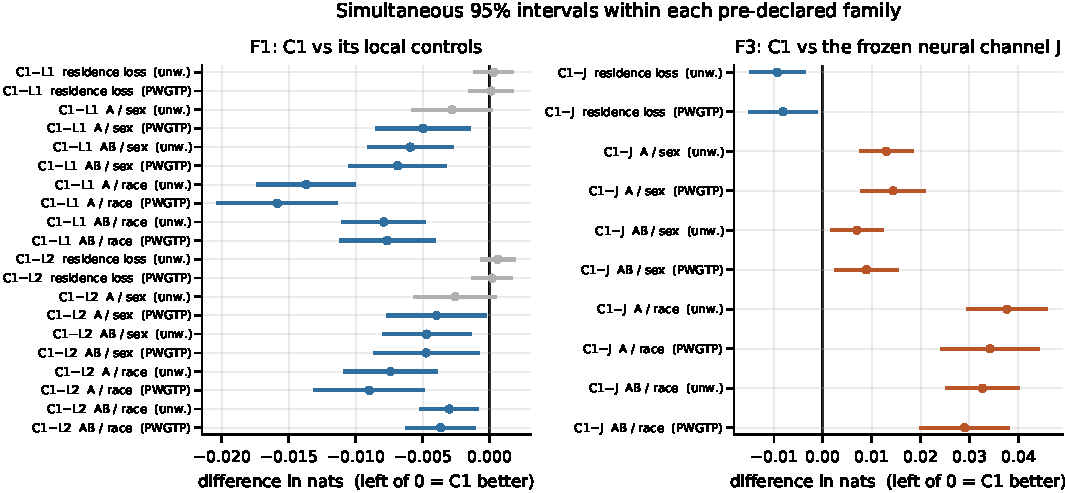
\includegraphics[width=\textwidth]{figures/forest_primary.pdf}
\caption{Paired differences with simultaneous 95\% intervals inside each pre-declared family, Mode B
(fresh 2017 attacks), unweighted and PWGTP. Each difference is candidate minus comparator in nats;
\textbf{left of zero means C1 is better} for every endpoint shown, including residence loss. Blue:
the interval lies entirely below zero. Orange: entirely above zero. Grey: it crosses zero, which
means the comparison is unresolved, \emph{not} that the endpoint is unaffected.}
\label{fig:forest}
\end{figure}

\begin{table}[t]
\centering\small
\begin{tabular}{llrrl@{\hspace{4pt}}c}
\toprule
Contrast & Endpoint & Estimate & Seeds 0 / 1 / 2 & Adjusted 95\% & \\
\midrule
\multicolumn{6}{l}{\textit{F1: coalition conditioning vs local controls} ($c=2.930$)} \\[1pt]
C1 $-$ L1 & residence loss & 0.00029 & 0.0005 / 0.0004 / -0.0001 & [-0.00118, 0.00176] &  \\
C1 $-$ L1 & A / sex & -0.00282 & -0.0046 / -0.0055 / 0.0017 & [-0.00585, 0.00020] &  \\
C1 $-$ L1 & AB / sex & -0.00593 & -0.0046 / -0.0094 / -0.0038 & [-0.00915, -0.00271] & $\blacktriangledown$ \\
C1 $-$ L1 & A / race & -0.01369 & -0.0145 / -0.0129 / -0.0137 & [-0.01737, -0.01002] & $\blacktriangledown$ \\
C1 $-$ L1 & AB / race & -0.00792 & -0.0054 / -0.0109 / -0.0075 & [-0.01105, -0.00478] & $\blacktriangledown$ \\
C1 $-$ L2 & residence loss & 0.00059 & 0.0012 / 0.0009 / -0.0004 & [-0.00073, 0.00191] &  \\
C1 $-$ L2 & A / sex & -0.00258 & -0.0020 / -0.0051 / -0.0007 & [-0.00568, 0.00052] &  \\
C1 $-$ L2 & AB / sex & -0.00472 & -0.0058 / -0.0060 / -0.0024 & [-0.00804, -0.00140] & $\blacktriangledown$ \\
C1 $-$ L2 & A / race & -0.00741 & -0.0054 / -0.0074 / -0.0095 & [-0.01088, -0.00394] & $\blacktriangledown$ \\
C1 $-$ L2 & AB / race & -0.00302 & 0.0004 / -0.0039 / -0.0056 & [-0.00524, -0.00081] & $\blacktriangledown$ \\
\addlinespace
\multicolumn{6}{l}{\textit{F3: coalition channel vs frozen neural channel} ($c=2.728$)} \\[1pt]
C1 $-$ J & residence loss & -0.00932 & -0.0141 / -0.0020 / -0.0118 & [-0.01500, -0.00363] & $\blacktriangledown$ \\
C1 $-$ J & A / sex & 0.01301 & 0.0201 / 0.0034 / 0.0155 & [0.00753, 0.01848] & $\blacktriangle$ \\
C1 $-$ J & AB / sex & 0.00697 & 0.0088 / 0.0014 / 0.0107 & [0.00151, 0.01242] & $\blacktriangle$ \\
C1 $-$ J & A / race & 0.03767 & 0.0428 / 0.0383 / 0.0320 & [0.02941, 0.04594] & $\blacktriangle$ \\
C1 $-$ J & AB / race & 0.03268 & 0.0330 / 0.0318 / 0.0332 & [0.02504, 0.04032] & $\blacktriangle$ \\
\addlinespace
\bottomrule
\end{tabular}

\caption{Primary comparisons, Mode B, scope \texttt{transport\_all}, budget 360, unweighted.
$\blacktriangledown$ marks an adjusted interval entirely below zero (candidate better),
$\blacktriangle$ entirely above (worse). The PWGTP rows are in Figure~\ref{fig:forest}.}
\label{tab:primary}
\end{table}

On the sealed 2017 partition, C1 has a simultaneous-interval advantage over both its equal-strength
local control L1 and the equal-total-mass control L2, under both weightings: 8 of 8 sensitive
endpoints better, 0 worse, critical value $2.9301$ over 20 endpoints. Frozen 2018 attacks reproduce
the ordering, so it is not an artifact of refitting attackers on the new year. This is the
coordination criterion development had failed, and the registered rule passed.

\subsection{The residence rule is a point criterion, and only a point criterion}

\begin{table}[t]
\centering\small
\begin{tabular}{llrrrrl}
\toprule
Contrast & Weight & Estimate & SE & Pointwise 95\% & Simultaneous 95\% & Non-inferior? \\
         &        &          &    & upper bound     & upper bound      & (margin $0.001$) \\
\midrule
C1 - L1 & unw. & 0.00029 & 0.00050 & \textbf{0.00112} & 0.00166 & no \\
C1 - L1 & PWGTP & 0.00010 & 0.00056 & \textbf{0.00103} & 0.00164 & no \\
C1 - L2 & unw. & 0.00059 & 0.00045 & \textbf{0.00135} & 0.00182 & no \\
C1 - L2 & PWGTP & 0.00017 & 0.00053 & \textbf{0.00102} & 0.00162 & no \\
\bottomrule
\end{tabular}

\caption{Retrospective non-inferiority for the F1 residence endpoint at the registered margin of
$0.001$ nats. Lower loss is better, so the question is whether the \emph{upper} bound falls below
$+0.001$. It does not, in any of the four comparisons, even under the most permissive procedure
(a pointwise one-sided bootstrap percentile with no multiplicity adjustment). This assessment is
retrospective and does not replace the registered outcome.}
\label{tab:equivalence}
\end{table}

The rule as implemented is $\text{seed-mean}(\text{C1}-\text{comparator})\le 0.001$ on the residence
log loss. It is one-sided---C1 may be arbitrarily better---and it is a \emph{point} criterion: no
interval enters it. The four values are $0.00029$, $0.00010$, $0.00059$, $0.00017$, so it passes, and
would pass under a two-sided reading too.

It does not follow that the residence cost is below $0.001$.
Table~\ref{tab:equivalence} shows that \textbf{zero of four comparisons support non-inferiority at
that margin}, missing it by 2\% to 35\%, and zero support two-sided equivalence. Our earlier phrasing
``inside the prespecified $0.001$ band'' invited exactly the interval reading the evidence does not
support, and we withdraw it (Section~\ref{sec:withdrawn}).

A related distinction: the advantage rule requires that \emph{no} sensitive endpoint is significantly
worse. That is an absence-of-evidence condition. Two F1 endpoints have adjusted intervals that cross
zero on the harmful side---C1 versus L1 on A/sex, $[-0.00585,+0.00020]$, and C1 versus L2 on A/sex,
$[-0.00568,+0.00052]$---so up to $5\times10^{-4}$ nats of \emph{extra} local sex recovery is not
excluded. The rule is satisfied; the endpoints are not shown to be unaffected.

\subsection{Absolute against additional recovery}

\begin{figure}[t]
\centering
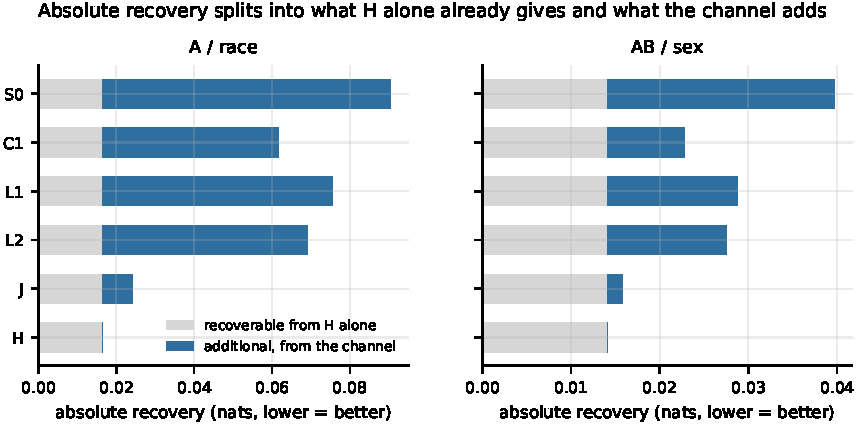
\includegraphics[width=\textwidth]{figures/absolute_vs_additional.pdf}
\caption{Absolute recovery on the 2017 final partition, split into the part an attacker already gets
from the published service alone (grey) and the part the appended channel adds (blue). Mode B,
unweighted, seed mean. Lower is better. The grey segment is identical across interfaces by
construction: it is H's own recovery.}
\label{fig:absadd}
\end{figure}

\begin{table}[t]
\centering\small
\begin{tabular}{lrrrrr}
\toprule
& residence & \multicolumn{2}{c}{A / race} & \multicolumn{2}{c}{AB / sex} \\
\cmidrule(lr){3-4}\cmidrule(lr){5-6}
Interface & gain vs H & absolute & additional & absolute & additional \\
\midrule
H & 0.0000 & 0.0165 & 0.0000 & 0.0141 & 0.0000 \\
J & 0.0189 & 0.0241 & 0.0076 & 0.0159 & 0.0017 \\
L1 & 0.0285 & 0.0754 & 0.0590 & 0.0288 & 0.0146 \\
L2 & 0.0288 & 0.0692 & 0.0527 & 0.0275 & 0.0134 \\
C1 & 0.0282 & 0.0617 & 0.0453 & 0.0228 & 0.0087 \\
S0 & 0.0304 & 0.0905 & 0.0740 & 0.0397 & 0.0256 \\
\bottomrule
\end{tabular}

\caption{Absolute and additional (H-relative) recovery beside residence gain. Mode B,
\texttt{transport\_all}, 360, unweighted, seed mean. Lower is better for recovery, higher for
residence gain.}
\label{tab:absadd}
\end{table}

The H baseline is substantial: an attacker on the bare service wire already recovers $0.0165$ nats of
A/race and $0.0141$ of AB/sex. Two consequences.

\emph{Ratios are scale-dependent; differences are not.} C1 against J on A/race is $6.0\times$ on
increments ($0.0453$ vs $0.0076$) and $2.6\times$ on absolute values ($0.0617$ vs $0.0241$). The
paired difference, $0.0377\,[0.0294, 0.0459]$, is identical on both scales, because the shared prior
and H selection cancel inside a paired contrast. We quote the difference.

\emph{Some increments are negative, and that is a measurement, not protection.} 22 of 429 unweighted
role-cells are negative in the primary scope. J's own A/sex increment is negative under PWGTP
($-0.0033$, interval excluding zero) and its absolute A/sex recovery, $0.0092$, is \emph{below} H's
own $0.0101$: the validation-selected fresh attack on J's wire does worse than H's attack. That is a
property of selection. H's attack, routed onto J's augmented wire, remains executable, so a negative
increment removes nothing an H-only attacker already had. In 8 of 312 sensitive cells the selected
attack generalises worse than that routed H control (15 of 312 under the fresh-only scope). Adding
frozen 2018 candidates lowers additional recovery for every interface because it strengthens the
subtracted baseline, not because the wire discloses less.

\subsection{The mechanism is not competitive}

C1 is significantly worse than J on \emph{all four} sensitive endpoints under \emph{both} weightings,
and worse on both source probes (income $+0.0081$, employment $+0.0135$, intervals excluding zero).
It is better only on residence, $-0.0093\,[-0.0150,-0.0036]$. Figure~\ref{fig:forest}, right panel.
This is the pre-declared secondary comparison and it fails; our earlier summary said it failed on
local race, which understated it.

``Same width'' is a \emph{capacity} control---both channels are 16-dimensional---and says nothing
about whether their utility is comparable. It is not.

\subsection{Matching the two channels on average utility}

\begin{figure}[t]
\centering
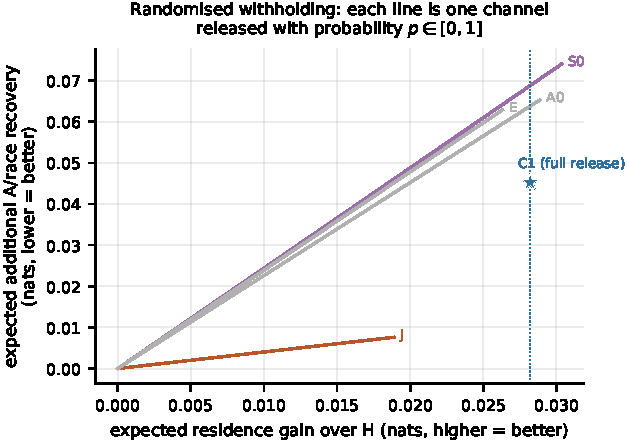
\includegraphics[width=0.56\textwidth]{figures/withholding.pdf}
\caption{Under the declared randomised-withholding mechanism (H always released; an independent
visible $\mathrm{Bernoulli}(p)$ branch, fixed per person, decides whether the channel is also
released), expected residence gain and expected additional recovery are both exactly $p$ times their
full-release values, so each channel traces a straight line from the origin. Lower and further right
is better. The dotted line marks C1's full-release residence gain: \textbf{J's line stops short of
it}, so no withholding schedule makes J as useful as C1. Where a comparator \emph{can} reach that
line (S0, A0), it sits above C1.}
\label{fig:withholding}
\end{figure}

\begin{table}[t]
\centering\small
\begin{tabular}{llrlr}
\toprule
Withheld channel & matched to & $p^\star$ & identifiable? & A/race at $p^\star$ \\
\midrule
E & C1 & 1.072 & \textbf{no} & --- \\
A0 & C1 & 0.976 & yes & 0.0638 \\
L025 & C1 & 1.615 & \textbf{no} & --- \\
L20 & C1 & 1.555 & \textbf{no} & --- \\
J & C1 & 1.493 & \textbf{no} & --- \\
S0 & C1 & 0.929 & yes & 0.0688 \\
\bottomrule
\end{tabular}

\caption{Post-hoc average-utility matching. $p^\star=\text{gain}_{\text{C1}}/\text{gain}_{\text{source}}$
is the withholding probability at which a channel's \emph{mean} residence gain equals C1's; it is
identified in closed form because the mixture is exactly linear in $p$. Values above 1 mean the
comparator cannot reach C1's utility at any schedule. The last column is the comparator's expected
additional A/race recovery at $p^\star$, to compare against C1's $0.0453$.}
\label{tab:matching}
\end{table}

Because the routed family mixes per-person \emph{losses}, expected residence gain over H is exactly
$p$ times the full-release gain, and expected additional recovery is exactly $p$ times the
full-release increment. The probability matching a target's \emph{mean} residence gain is therefore
identified in closed form. This yields two findings the fixed-$p$ grid did not surface.

First, \textbf{J cannot be made as useful as C1 by any withholding schedule}: it would need
$p^\star=1.49$. Nor can E ($1.07$), L025 ($1.62$) or L20 ($1.56$). The C1-versus-J comparison is not
two points on one traversable frontier. Second, \textbf{the ordering survives matching in both
directions}. Where matching is identifiable, C1 beats withheld A0 ($p^\star=0.976$) and withheld S0
($p^\star=0.929$) on all four sensitive endpoints; and C1 withheld down to J's residence level
($p^\star=0.670$) still leaks far more than J on all four ($0.0303$ against $0.0076$ on A/race).

Both statements are \textbf{post-hoc average-utility matching}: $p^\star$ is estimated from the same
data as the outcome, so the fixed-$p$ intervals do not transfer to it, and it matches an average over
people who receive different information. The original fixed-$p$ analysis is unchanged, and on it
neither family robustly dominates: withholding dominates a given spectral arm in 1--3 of 180 fixed
comparisons and a spectral arm dominates withholding in 0--3 of 180. A finite list of controls
failing to dominate C1 is not evidence that C1 is efficient.

\subsection{Service parity, probe quality, and what moved}

\begin{table}[t]
\centering\small
\begin{tabular}{lrrrr}
\toprule
& \multicolumn{2}{c}{source-probe allowance} & \multicolumn{2}{c}{half-headroom} \\
\cmidrule(lr){2-3}\cmidrule(lr){4-5}
Interface & fresh (B) & frozen (A) & fresh (B) & frozen (A) \\
\midrule
H & 3/3 & 3/3 & 0/3 & 0/3 \\
J & 3/3 & 3/3 & 0/3 & 0/3 \\
L1 & 3/3 & 0/3 & 1/3 & 0/3 \\
L2 & 3/3 & 0/3 & 1/3 & 0/3 \\
C1 & 3/3 & 0/3 & 1/3 & 0/3 \\
S0 & 3/3 & 0/3 & 1/3 & 2/3 \\
\bottomrule
\end{tabular}

% counts are PASSING seeds out of 3.

\caption{Passing seeds out of 3 for the two reference criteria, unweighted. The legacy source-probe
allowance passes everywhere under fresh adaptation (B) but \textbf{passes in only 0--1 of 3 seeds for
every spectral arm under frozen transfer} (A): a frozen 2018 probe does not carry onto a spectral
wire in a new year, and refitting the probe repairs it. The released service vectors are identical
bits in all cases; a worse probe does not change a delivered prediction.}
\label{tab:criteria}
\end{table}

Three different objects must be kept apart. The \emph{released} income, employment and coverage
probability vectors are identical, bitwise, in every condition---structural, verified on 210 of 210
released views. Service \emph{accuracy} changes with the year: employment $+0.0138$ nats, income
$-0.0145$, coverage $-0.0067$. Independently fitted \emph{source probes} are a third thing again, and
their pass pattern separates the two modes (Table~\ref{tab:criteria}).

\subsection{Development against transport: magnitude, not only resolution}

\begin{figure}[t]
\centering
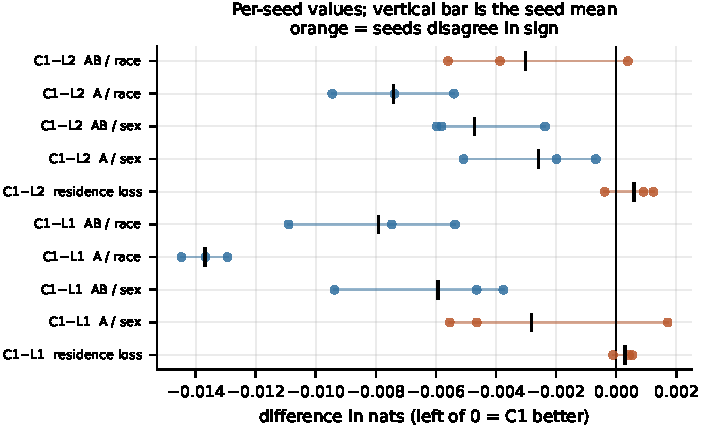
\includegraphics[width=0.62\textwidth]{figures/per_seed.pdf}
\caption{The three per-seed values behind each F1 endpoint (unweighted); the vertical bar is the
seed mean that enters the estimand. Orange marks endpoints where the seeds do not all share the
seed-mean sign. Aggregate sign agreement can conceal per-seed disagreement, and does here.}
\label{fig:perseed}
\end{figure}

All 20 F1 \emph{seed-mean} signs agree with development. Only 13 of 20 agree in \emph{every seed}
(Figure~\ref{fig:perseed}); across all 90 family endpoints only 48 of 90 have all three seeds
agreeing with their own seed mean. And magnitudes moved: F1 point estimates changed by factors
between $0.054\times$ and $14.8\times$ (for instance C1 $-$ L2 on AB/sex went from $-0.0003$ to
$-0.0047$). A larger evaluation pool shrinks standard errors; it does not move point estimates by a
factor of fifteen. The years differ in sample size, in calendar year, in evaluation pool and in which
attacker families were available, and this design does not separate them. Our earlier claim that
``what changed is resolution, not direction'' is withdrawn.

\subsection{Support limitations}

Race class 3 (Alaska Native alone) has one person in the final partition and none in 2017 attacker
validation, so class-specific recall and AUROC are undefined for it. Full nine-class log loss is
always scored with a fixed $10^{-12}$ probability floor and renormalisation; no category is dropped.
A comparable-category diagnostic restricted to classes supported in every fitting pool of both modes
reproduces the F1 race differences almost exactly (C1 $-$ L1 on A/race: $-0.0137$ against $-0.0137$
on all rows). \textbf{A class without support is unmeasured, not protected.}

\section{Claims this revision withdraws or narrows}
\label{sec:withdrawn}

Stated explicitly, because each was in our own earlier draft.

\begin{enumerate}\itemsep1pt
\item ``\emph{Residence difference inside the prespecified $\pm0.001$ band.}'' The rule is one-sided
and applies to a point estimate. Zero of four interval comparisons support non-inferiority at that
margin (Table~\ref{tab:equivalence}). The registered rule still passed.
\item ``\emph{What changed is resolution, not direction.}'' Magnitudes changed by $0.054\times$ to
$14.8\times$; sample size alone does not explain the newly significant result.
\item ``\emph{Every F1 endpoint keeps its development sign (20/20).}'' True of seed means; 13 of 20
in every seed.
\item ``\emph{C1 versus J fails on local race.}'' It fails on all four sensitive endpoints under both
weightings, plus both source probes.
\item ``\emph{Several times more sex and race.}'' Scale-dependent: $6.0\times$ on increments,
$2.6\times$ in absolute terms. We now quote the paired difference.
\item ``\emph{Under frozen transfer every spectral arm fails in 0--1 of 3 seeds.}'' The underlying
column counts \emph{passing} seeds; the arms pass in 0--1 of 3, i.e.\ fail in 2--3 of 3. The
published table was correct and the sentence inverted it.
\item ``\emph{The gap is the surrogate, not the solver.}'' Global optimality of the fixed matrix
excludes a solver failure and nothing else. Five candidate causes---the finite feature map, nuisance
misspecification, the normalisation, the fixed rank, the reconstruction surrogate, and finite-sample
generalisation---remain unseparated. We now say ``consistent with''.
\item ``\emph{If a nonlinear penalty also loses, the conclusion generalises to the closed-form
spectral family.}'' Withdrawn entirely. Two arms failing is evidence about two arms; and a penalty
acting on nonlinear functions of $Z$ is provably not a trace form $\operatorname{tr}(W^\top AW)$ for
any $W$-independent $A$---it is not invariant under $W\mapsto WQ$ for orthogonal $Q$, while every
trace form is---so such a successor is not in that family at all.
\item ``\emph{Two lock amendments.}'' Three exist. All are code-only; the third post-dates every
final-partition read.
\item \emph{Reporting the H-relative residence gain without the half-headroom failure.} Corrected in
Table~\ref{tab:criteria}.
\end{enumerate}

\section{Limitations}
\label{sec:limitations}

Three seeds are three fixed fitted systems on one cohort, not population replications. The bootstrap
covers people in the 2017 final partition only: it is not retraining variability and not a
Census-design variance, and PWGTP replicate weights were not used. Attack strength is a floor, not a
guarantee: every recovery number is what the tested families achieved. Only recipient A receives a
channel. Transport is between public survey years of the same state and age band, and cross-year
person distinctness cannot be established from public identifiers. Income is nominal and unadjusted.
The evaluation refits attackers but not the representation, so it does not test a mechanism retrained
on the new year. The 2018 pools have been used repeatedly across this line of work and are
development, not confirmation.

\textbf{Numerical recovery.} Three code-only lock amendments are recorded. The first fixed a
release-file write race; the second fixed rare load-dependent prediction corruption found by an
independent cross-process replay; the third changed three published tables from CSV to gzip CSV and
post-dates every final read. Machine memory pressure was the \emph{observed condition} under which
the corruption appeared; it is not a demonstrated cause, and we do not claim one. The repair does not
depend on the diagnosis: every prediction is now computed twice and must agree, all final units were
rescored, originals are preserved, and the post-fix replay found 0 mismatches in 59{,}874 predictions
with 0 selection changes in 37{,}122 validation predictions.

\section{Conclusion}
\label{sec:conclusion}

A service that has already published predictions can add a reusable channel beside them without
changing a single released number, and can steer that channel away from directions a recipient or a
colluding pair would use to infer sex and race. On a locked, previously unused survey year, the
coalition-conditioning knob does what it claims against both of its local controls, under
simultaneous intervals and both weightings. It also costs residence utility by an amount the data
cannot bound below the $0.001$ nats our registered rule used, and the channel it steers remains
significantly worse than a frozen adversarially trained channel of the same width on every sensitive
endpoint---an ordering that survives matching the two on average utility in both directions.

The defensible contribution is the problem formulation and the evaluation design: fixed published
outputs as a hard constraint, recipient-specific and coalition-specific audit roles, fresh and frozen
attackers never pooled, absolute and incremental recovery reported side by side, negative increments
retained unclipped, and a sealed temporal transport with the multiplicity fixed in advance. The
method result is negative and we report it as such.

\section{Reproducibility}
\label{sec:repro}

Deterministic seeds throughout; every unit writes a hash-bound completion record; the lock refuses to
open the final partition if any hashed input changed. All 90 pre-declared endpoints in this paper
were regenerated from stored per-person predictions by an independently written scorer that shares no
computation function with the original report code, agreeing to $1.1\times10^{-15}$ on point
estimates and $2.4\times10^{-15}$ on interval endpoints, with identical critical values; candidate
selection was re-derived from stored validation losses with 0 mismatches in 924 cells; and the lock
was re-verified over all 17{,}639 hashed inputs with every amendment applied. Commands, file map and
software versions: \texttt{REPRODUCE.md}. Fitted objects, releases and per-person arrays stay local;
compact aggregates, code, tables and figures are published.

\bibliography{references}

\end{document}
